\thispagestyle{quantoannone}
\pagestyle{quantoan}
\everymath{\color{quantoan}}
\graphicspath{{../quantoan/pic/}}
\blfootnote{\color{quantoan}\color{quantoan}$^*$Theo The Economist.}
\blfootnote{\color{quantoan}\color{quantoan}$^1$Đại học Sư phạm Hà Nội.}
\begingroup
\AddToShipoutPicture*{\put(0,616){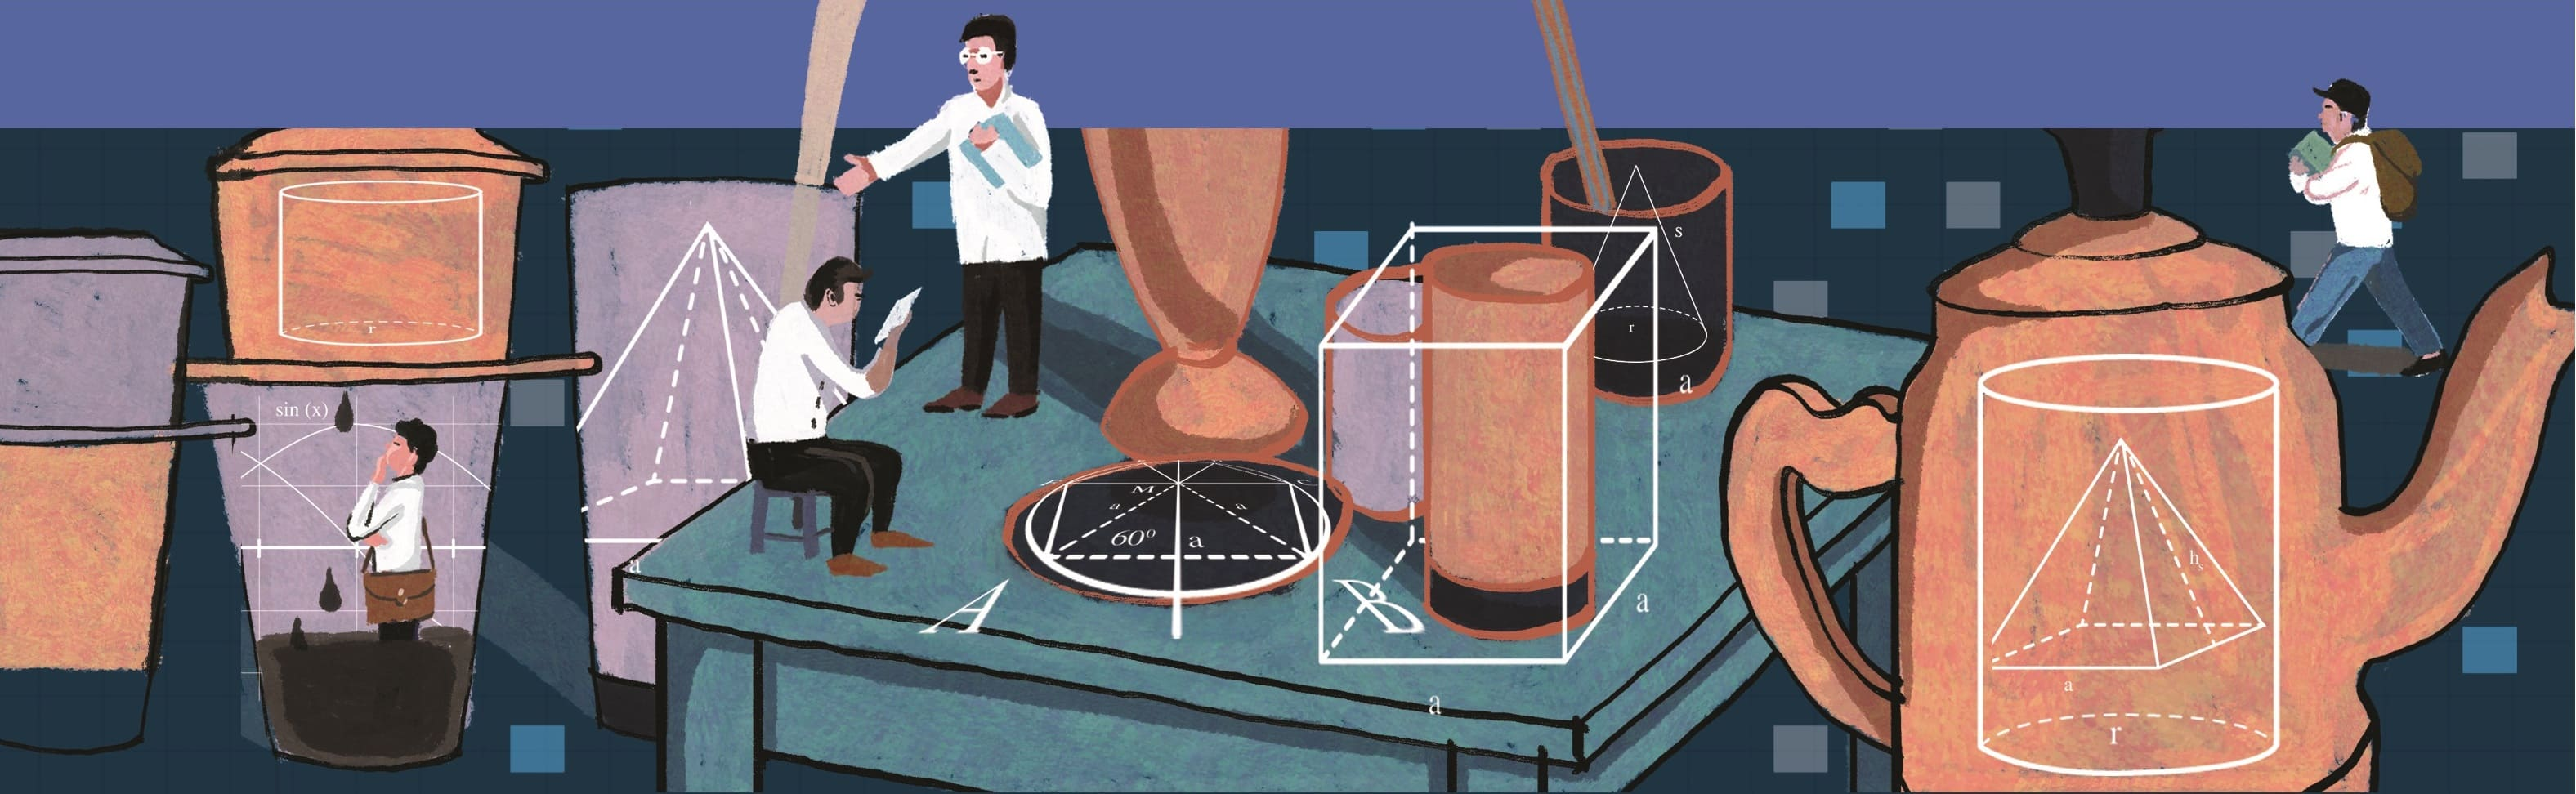
\includegraphics[width=19.3cm]{../bannerquantoan}}}
\AddToShipoutPicture*{\put(126,520){
\includegraphics[scale=1]{../tieude3.pdf}}}
\centering
\endgroup

\vspace*{185pt}

%\newpage
%\blfootnote{\color{quantoan}\color{quantoan}$^1$Đại học Sư phạm Hà Nội.}
%\begingroup
%\AddToShipoutPicture*{\put(120,675){
\includegraphics[scale=1]{../tieude3.pdf}}}
%\centering
%\endgroup
%
%
%\vspace*{35pt}

\begin{multicols}{2}
	Có một truyền thuyết  kể rằng thành phố Portland, bang Oregon đã suýt được gọi là Boston. Cuối cùng thì vấn đề đã được quyết định nhờ một cuộc tung đồng xu được tổ chức vào năm $1845$ giữa Francis Pettygrove, người đến từ một thành phố Portland khác, ở bang Maine, và Asa Lovejoy, đến từ Boston (ở bang Massachusetts). Nhưng mọi chuyện có thể đã khác đi, theo Frantisek Bartos, một sinh viên tốt nghiệp tại Đại học Amsterdam, nếu con người chúng ta  không phải là những người tung xu một cách lưỡng lự thiếu dứt khoát như vậy.
	\begin{figure}[H]
		\vspace*{-5pt}
		\centering
		\captionsetup{labelformat= empty, justification=centering}
		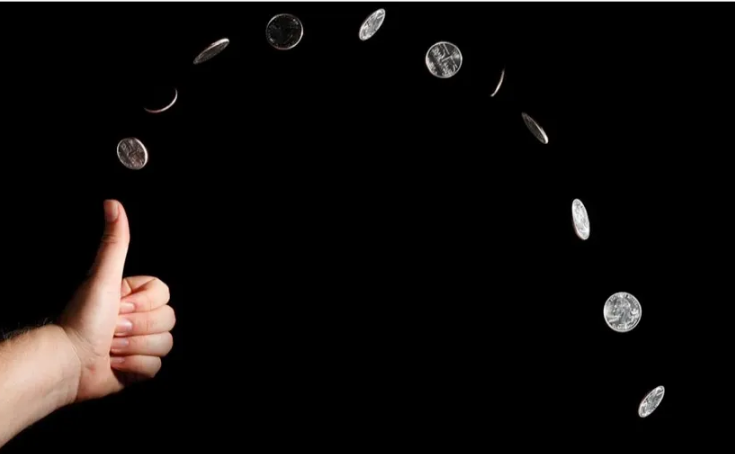
\includegraphics[width= 1\linewidth]{1111}
%		\caption{\small\textit{\color{}}}
		\vspace*{-15pt}
	\end{figure}
	Bartos đã quan tâm đến một dự đoán hấp dẫn của Persi Diaconis, Susan Holmes và Richard Montgomery, một nhóm các nhà toán học người Mỹ. Trong một bài báo đăng vào năm $2007$, bộ ba này đã phân tích tính chất vật lý của việc tung đồng xu và nhận thấy có một điều gì đó khá hấp dẫn. Bên cạnh việc khiến đồng xu quay lộn nhào, hầu hết mọi người đều có xu hướng tạo ra một sự xoay nhẹ cho đồng xu khi họ tung nó. Điều đó làm cho trục xuay mà đồng xu lật quanh đó sẽ bị trôi đẩy khi nó ở trên không trung, một hiện tượng gọi là tuế sai.
	\vskip 0.1cm
	Kết quả cuối cùng, khi các con số được xử lý, là: một đồng xu do con người ném sẽ thể hiện một xu hướng thiên lệch khá tinh tế nhưng bền vững. Tiến sĩ Diaconis và các đồng nghiệp của ông tính toán có khoảng $51\%$ khả năng một đồng xu sẽ rơi theo hướng như trước khi được ném. Nói cách khác, nếu nó ngửa trong tay người ném, có nhiều khả năng hơn một chút là nó cũng sẽ chạm đất ngửa. Hoặc ít nhất, đó cũng là dự đoán.
	\vskip 0.1cm
	Bartos cùng với sự nhiệt tình đáng ngưỡng mộ của mình bắt tay vào kiểm tra thực nghiệm. Anh đã tập hợp được $48$ tình nguyện viên và thuyết phục họ thực hiện (và có quay phim) $350{.}707$ lần tung đồng xu, sử dụng hàng chục đồng xu khác nhau, từ đồng hai rupee của Ấn Độ đến đồng xu hai franc Thụy Sỹ. Dĩ nhiên, dữ liệu của anh  đã xác nhận những gì vật lý đã dự đoán. Các đồng xu đã chạm đất cùng với mặt khi tung lên tới tận $50,8\%$ số lần được ném.
	\vskip 0.1cm
	Số liệu thống kê chỉ ra rằng bản thân các đồng xu không có sự thiên lệch cụ thể nào. Yếu tố quyết định thực sự là con người chúng ta rõ ràng không có khả năng ném thẳng.  Bartos không phải là người đầu tiên thu thập số liệu thống kê về việc tung đồng xu. Nhưng anh ta là người đầu tiên làm được điều đó ở quy mô đủ lớn để phát hiện ra sự thiên lệch. (Một nỗ lực trước đó gồm $40{.}000$ lần tung, do hai sinh viên tại Đại học California tại Berkeley  thực hiện, đã thiếu sức mạnh thống kê để xác nhận được  lý thuyết.)
	\vskip 0.1cm
	Cơ hội $50,8\%$ chỉ khác một chút so với mức công bằng hoàn hảo. Nhưng  Bartos chỉ ra rằng cơ hội đó lớn hơn cả  lợi thế mà một sòng bạc có được trong hầu hết các loại kiểu chơi blackjack. Và trong một số tình huống cơ hội đó có thể có vai trò quan trọng. Vào năm $2019$, Sue Cudilla trở thành thị trưởng của Araceli, một thị trấn ở Philippines, nhờ việc tung đồng xu sau khi cuộc bầu cử được tuyên bố là bất phân thắng bại. Quan trọng hơn nữa, việc tung đồng xu có thể xác định ai là người ném bóng hoặc đánh bóng trước trong môn cricket. Các vận động viên chuyên nghiệp luôn chi hàng nghìn đô--la  và hàng giờ tập luyện để tìm kiếm được những lợi thế cận biên. Có lẽ họ giờ  sẽ phải nên chú ý nhìn vào đồng xu lẻ trong túi quần của trọng tài.
\end{multicols}